\chapter{A review of the literature}

\section{Flow induced vibrations}
\label{sec:flow induced vibrations}


\section{Fluid-elastic galloping}
\label{fluid-elastic galloping}

Fluid-elastic galloping is one of the common observable flow-induced vibration on a slender body. This is because this phenomenon is most common in civil structures, such as buildings and iced-transmission lines, the term ``aeroelastic galloping" is commonly used as the body is driven by wind. However, this mechanism can occur on a slender body immersed in any fluid Newtonian fluid, provided that the conditions to sustain the galloping mechanism are satisfied. This work is based on a general Newtonian flow,thus the term `` fluid-elastic galloping" is used throughout this thesis.
   

\subsection{Excitation of galloping}
\label{sec:exci-galloping}

\citet{Paidoussis2010} describes galloping as a ``velocity dependent and damping controlled" phenomenon. Therefore, in order for a body to gallop, an initial excitation has to be given to that body. While this excitation is mainly caused by the force crated from vortex shedding, other fluid instabilities may contribute to this initial excitation.  When a bluff body moves along the transverse direction of the fluid flow, it generates a force along the transverse direction. This force, also known as the induced lift and is a resultant of the fluid flow and the motion of the body. When this body is attached to an flexible system (i.e. a system that can be modeled by a spring, mass and damper), the induced lift becomes the periodic forcing of the system. Galloping is sustained  if the induced lift is in phase with the motion of the body. This could be explained further by using a square cross section as an example.

\begin{figure}
\setlength{\unitlength}{\textwidth}

  \begin{picture}(1,0.23)(0,0.74)
    
  \put(0.2,0.76){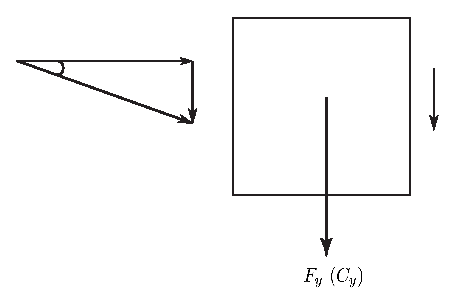
\includegraphics[width=0.5\unitlength]{../FnP/gnuplot/setup-1.eps}}         
      
      
   
 	\put(0.315,0.93){$U$}
 	\put(0.3,0.84){$U_i$}
    \put(0.42,0.88){$\dot{y}$}
    \put(0.28,0.895){ $\theta$}
    \put(0.7,0.87){\small $(+)$}
      	

 	
 	 

     

  \end{picture}

 \caption{Induced angle of attack on the square prism due to the resultant of free-stream velocity of the fluid and transverse velocity of the body.}
    \label{fig:setup_1}
\end{figure}

 Figure \ref{fig:induced_lift_sketch}  illustrates the motion of the body at a given instantaneous time.The induced angle of attack is formed on the square cross section as a result of the free stream velocity vector $U$ and the transverse velocity vector of the body $\dot{y}$. Thus, a force is formed in phase with the motion of the body for the case of a square cross section. This mechanism could also be observed on other bodies which are prone to galloping. The sign convention in this figure (and generally used in this scope of research) states that downward direction is positive. Hence, the force generated on a body under the influence of galloping, could be also identified as a ``negative lift".
 

\subsection{Quasi-steady state theory}
\label{sec:QSS theory}


According \cite{Paidoussis2010},the initial studies by \cite{Glauert1919} provided a criterion for galloping by considering the auto-rotation of a stalled aerofoil. As this phenomenon commonly occur in iced transmission lines, \cite{DenHartog1956} has provided a theoretical explanation for iced electric transmission lines. 

The pioneering study that mathematically models galloping was conducted by \cite{Parkinson1964}. This model has been widely used in almost all subsequent studies on galloping. A weakly non-linear oscillator model was developed by in that study to predict the response of the system. Essentially the quasi-steady assumption was made to develop this model. This assumes that the instantaneous induced lift force of the oscillating body is equal to that of the lift force generated by the same body at the same induced angle of attack. For the quasi-steady assumption to be valid, the conditions below have to be satisfied.

\begin{itemize}
 \item The velocity of the body does not change rapidly
 \item There is no interaction between vortex shedding and galloping
\end{itemize}

The second condition is satisfied by ensuring the vortex shedding frequency is much higher than the galloping frequency.
The oscillator equation was solved using the Krylov and Bogoliubov method \citep{Parkinson1964}. Details of this method is not included in this thesis because this study uses numerical intergration instead. The results obtained form experiments, carried out at $\reynoldsnumber=2200$ and a mass ratio (\mstar) around 1164 had a good agreement with the theoretical data which is shown in figure \ref{fig:parkinson_paper_data}.

\begin{figure}
	
  \setlength{\unitlength}{\textwidth}

        \begin{picture}(1,0.82)(0,0.4)

      % % % Parkinson Data 

      \put(0.05,0.39){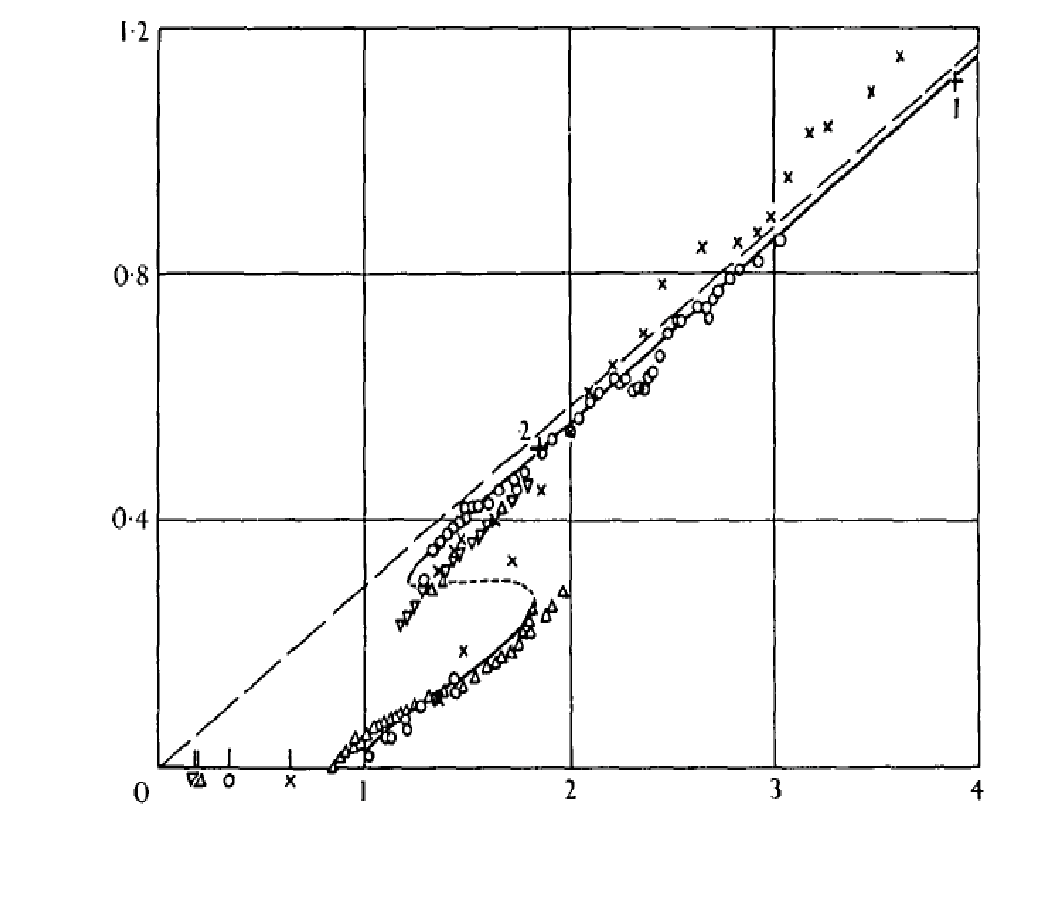
\includegraphics[width=0.9\unitlength]{./chapter-literature-revirw/fnp/parkinson_data.eps}}
      
%       \put(0.07,0.95){$\displaystyle\frac{V}{D}$}
%       \put(0.07,1.3){$\displaystyle\frac{A}{D}$}
       \put(0.05,0.8){\Large$\frac{nA}{2\beta}\bar{Y}_s$}
       \put(0.52,0.42){\Large$\frac{nA}{2\beta}U$}
       \
%\put(0.189,1.415){\small(a)}
%\put(0.189,1.07){\small(b)}
%\put(0.189,0.73){\small(c)}

%  


    \end{picture}

  \caption{``Collapsed amplitude-velocity characteristic. Theory: \solidrule \ stable limit cycle, \dashedrule unstable limit cycle. Experiment $\times \ \beta = .00107$, $\circ \ \beta =.00196$,\ $\vartriangle \beta=.00364$,$\triangledown \ \beta = .00372$,\ $+1 \ \beta=.0012$,\ $+2 \ \beta=.0032$ Reynolds numbers $4,000-20,000$ ". Figure extracted from \cite{Parkinson1964}. $\frac{nA}{2\beta}\bar{Y}_s$ is the dimensionless displacement amplitude parameter and $\frac{nA}{2\beta}U$ is the reduced velocity.$\beta$ is the damping ratio and $n=\frac{1}{\mstar}$. The experimental data shows a good agreement with the theoretical model.}
    \label{fig:parkinson_paper_data}
\end{figure}

 %vspace{10cm}


\subsubsection*{Quasi-steady state oscillator model}

The equation of motion of transversely oscillating body is given by 
\begin{equation}
\label{equationofmotion}
m\ddot{y}+c\dot{y}+ky=F_y,
\end{equation}
where the forcing term $F_y$ is given by
\begin{equation}
\label{lift equation}
F_y=\frac{1}{2}\rho U^2\mathcal{A}C_y.
\end{equation}

As explained previously, the quasi-steady assumption uses the stationary $C_y$ data (which consists of both lift and drag components) for varying angles of attack as inputs to the oscillator equation.\citet{Parkinson1964} used a $7^th$ order odd interpolating polynomial to interpolate the $C_y$ data. The order of the polynomial can be chosen arbitrarily depending on the study. For example \citet{Barrero-Gil2009,Barrero-Gil2010a} have used a $3_{rd}$ order polynomial in order to simplify the analytical model. However, \citet{Ng2005} pointed out that a $7_{th}$ order polynomial is sufficient as higher order polynomials do not provide significantly better result.    

\begin{equation}
\label{cy ploynomial}
C_y(\theta)=a_1\left(\frac{\dot{y}}{U}\right)-a_3\left(\frac{\dot{y}}{U}\right)^3+a_5\left(\frac{\dot{y}}{U}\right)^5-a_7\left(\frac{\dot{y}}{U}\right)^7.
\end{equation}

Therefore by substituting the forcing function to the oscillator equation (Eq:\ref{equationofmotion}) the Quasi-steady state (QSS) model could be obtained (Eq:\ref{final_equation_motion}). 

\begin{equation}
\label{final_equation_motion}
m\ddot{y}{+}c\dot{y}{+}ky{=}\frac{1}{2}\rho U^2 \mathcal {A} \Bigg(a_1\left(\frac{\dot{y}}{U}\right){-}a_3\left(\frac{\dot{y}}{U}\right)^3{+}a_5\left(\frac{\dot{y}}{U}\right)^5{-}a_7\left(\frac{\dot{y}}{U}\right)^7 \Bigg).
\end{equation}

As the current study is focused on the low \reynoldsnumber region, it is a known fact that the vortex shedding will be correlated well and therefore provide a significant forcing. \citet{Joly2012} introduced and additional sinusoidal forcing function to the model in order to integrate the forcing by vortex shedding. By the addition of this forcing \citet{Joly2012} managed to obtain accurate predictions of the displacement amplitude even at low mass ratios, where the galloping is significantly suppressed by the vortex shedding to the point that it is no longer detectable. However, the strength or the amplitude of this sinusoidal forcing has to be tuned in an \emph{ad hoc} manner, and it was not clear the relationship between this forcing with the other system parameters. Thus in the current study this forcing was not used.

\subsubsection*{Presence of hysteresis}

Hysteresis could be observed in the amplitude data of \cite{Parkinson1964}. In contrast, the studies carried out by \citet{Barrero-Gil2009} and \citet{Joly2012} at much lower Reynolds numbers ($159\leq \reynoldsnumber\leq 200$), did not show any hysteresis. \citet{Luo2003} concluded that the hysteresis was present due to the presence of an inflection point in the $C_y$ curve at high Reynolds numbers (\citet{Parkinson1964} data) which was not present at lower Reynolds numbers. It was further explained and demonstrated by Luo that the inflection point occurs due to the intermittent re attachment of the shear layer in certain angles at high Reynolds numbers. 

\begin{figure}
	
  \setlength{\unitlength}{\textwidth}

  \begin{picture}(1,0.9)(0,0.75)

      % % % Parkinson Data 

      \put(-0.15,0.2){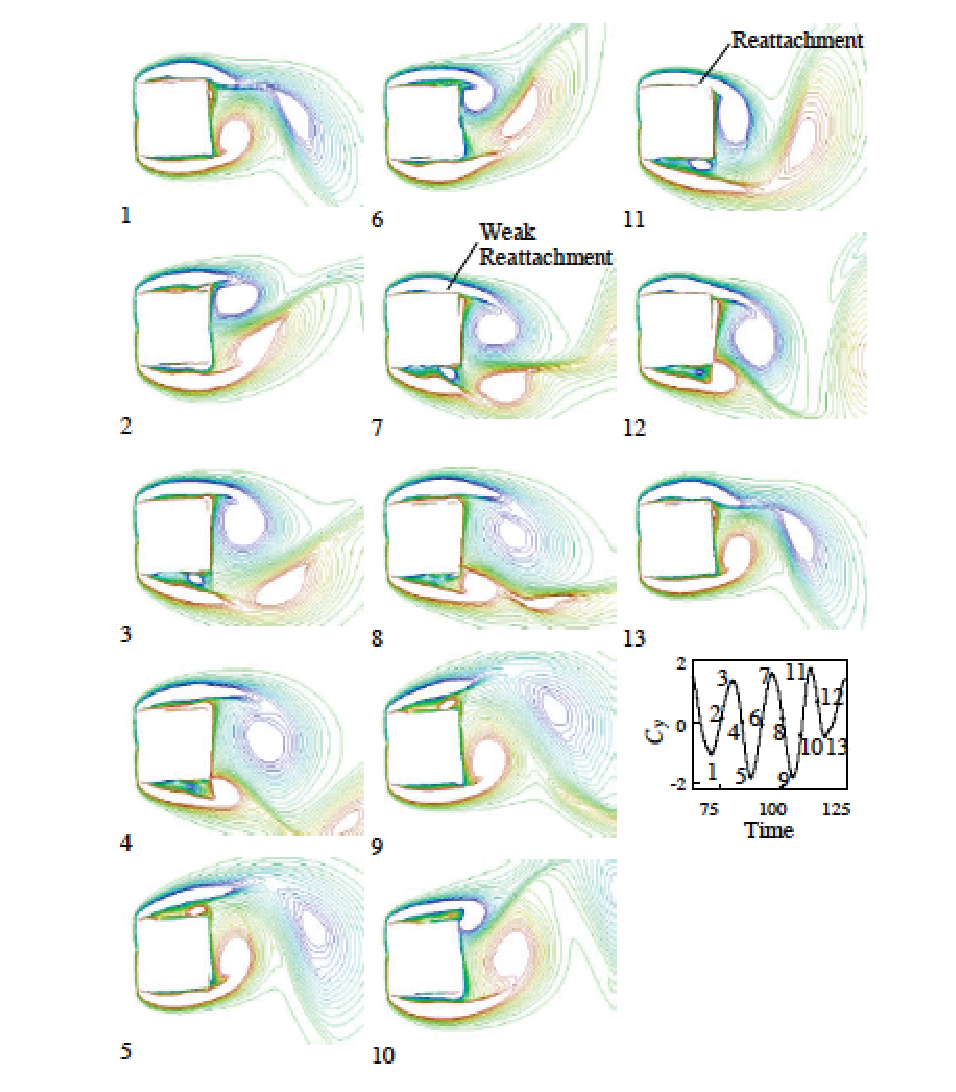
\includegraphics[width=1.3\unitlength]{./chapter-literature-revirw/fnp/luo-re-attachment.eps}}
      
%       \put(0.07,0.95){$\displaystyle\frac{V}{D}$}
%       \put(0.07,1.3){$\displaystyle\frac{A}{D}$}
      
%\put(0.189,1.415){\small(a)}
%\put(0.189,1.07){\small(b)}
%\put(0.189,0.73){\small(c)}

%  


    \end{picture}

  \caption{\label{fig:lit-review-luo-reattachment-1}Vorticity contours of \cy\ and the corresponding time for $\reynoldsnumber=1000$, $\theta=2^{\circ}$ extracted from \citet{Luo2003}. The intermittent shear level is visible in points 7 and 11}
\end{figure}


 %vspace{10cm}


Figure \ref{fig:lit-review-luo-reattachment} shows the vorticity contours of a square cross section obtained at various points of the vortex shedding cycle, at $\reynoldsnumber=1000$, $\theta=2^{\circ}$ obtained from \citet{Luo2003}. The points 7 and 11 shows the intermittent shear layer reattachment which causes the hysteresis in the \cy\ vs. $\theta$ curve at high Reynolds numbers.

\vspace{20mm}   

\subsection{Induced force and the shear layers}
\label{subsec:c_y and shear layers}

It is important to have an understanding on how the induced lift is generated from a fluid dynamics prespective. The quasi-steady model has already been validated and re-validated by many studies \citep{Parkinson1964,Barrero-Gil2009,Luo2003}, therefore the flow-field data of static body simulations could be used to analyse the underpinning fluid dynamic mechanisms governing galloping.

\begin{figure}[t!]

  \setlength{\unitlength}{\textwidth}

  \begin{picture}(1,0.35)(0,0.725)

    \put(-0.01,0.76){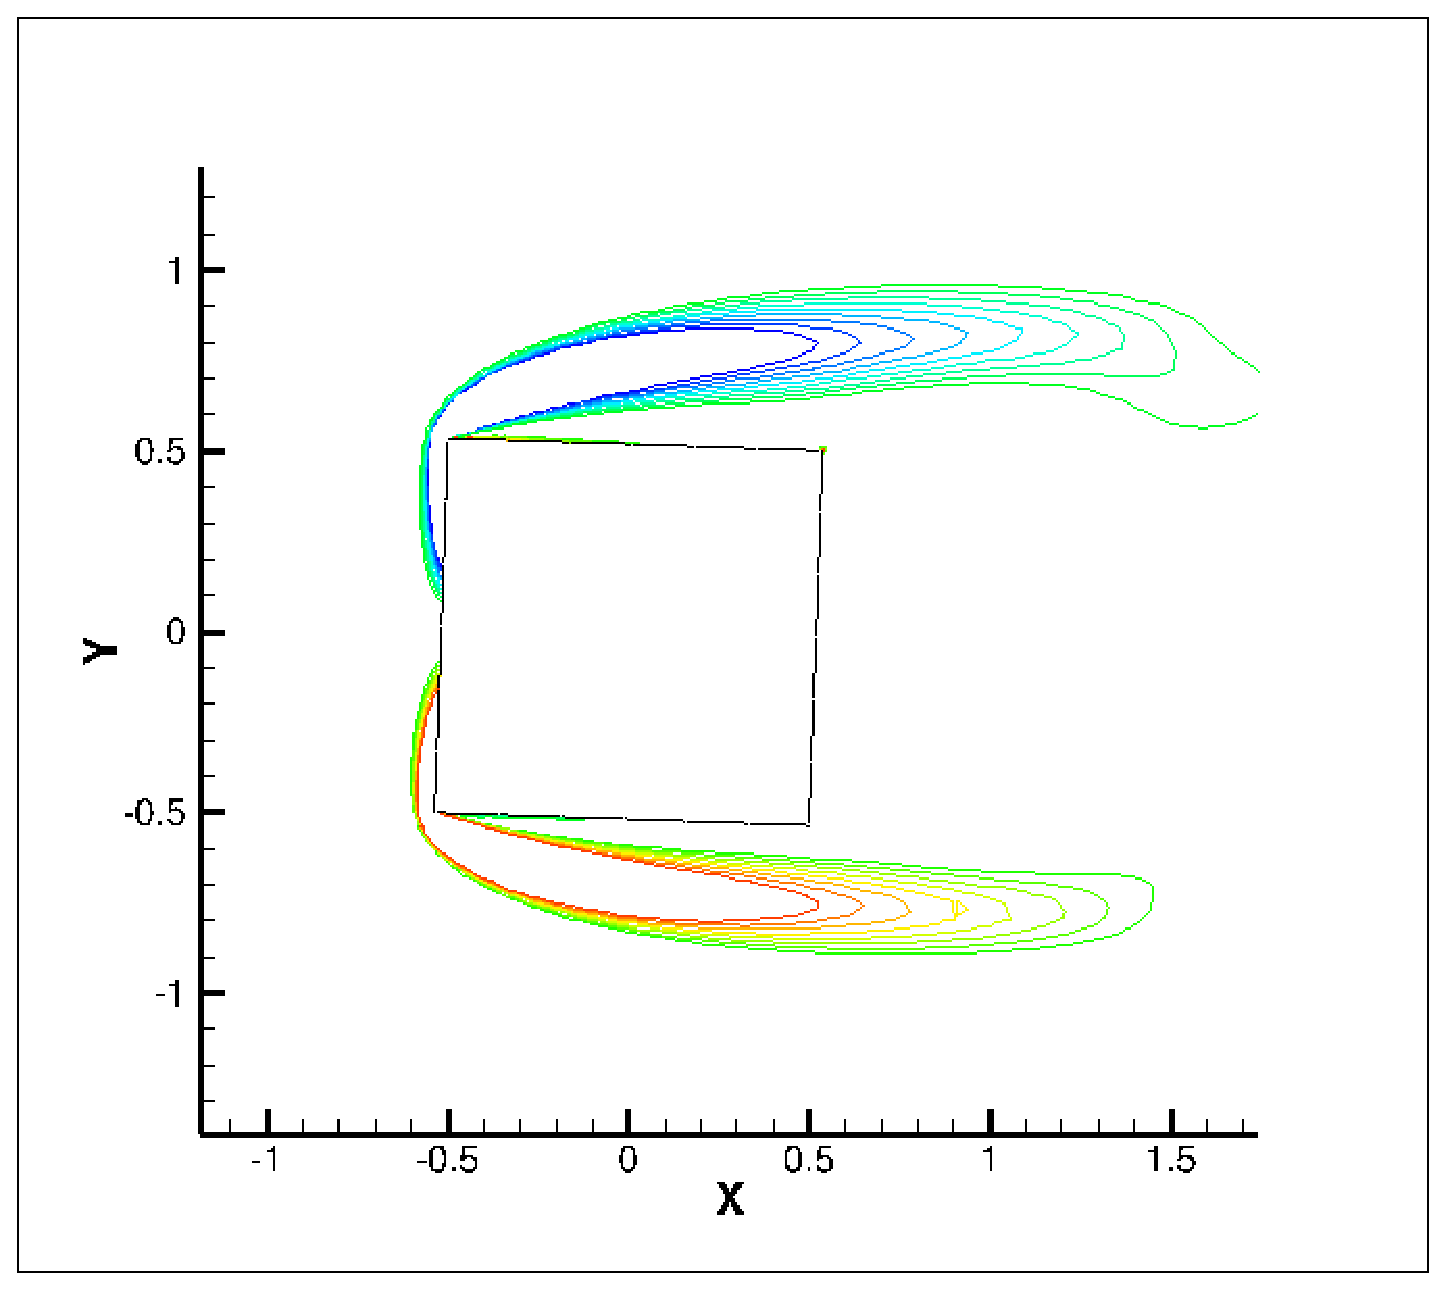
\includegraphics[width=0.33\unitlength]{./chapter-literature-revirw/fnp/square-2.eps}}
    \put(0.335,0.76){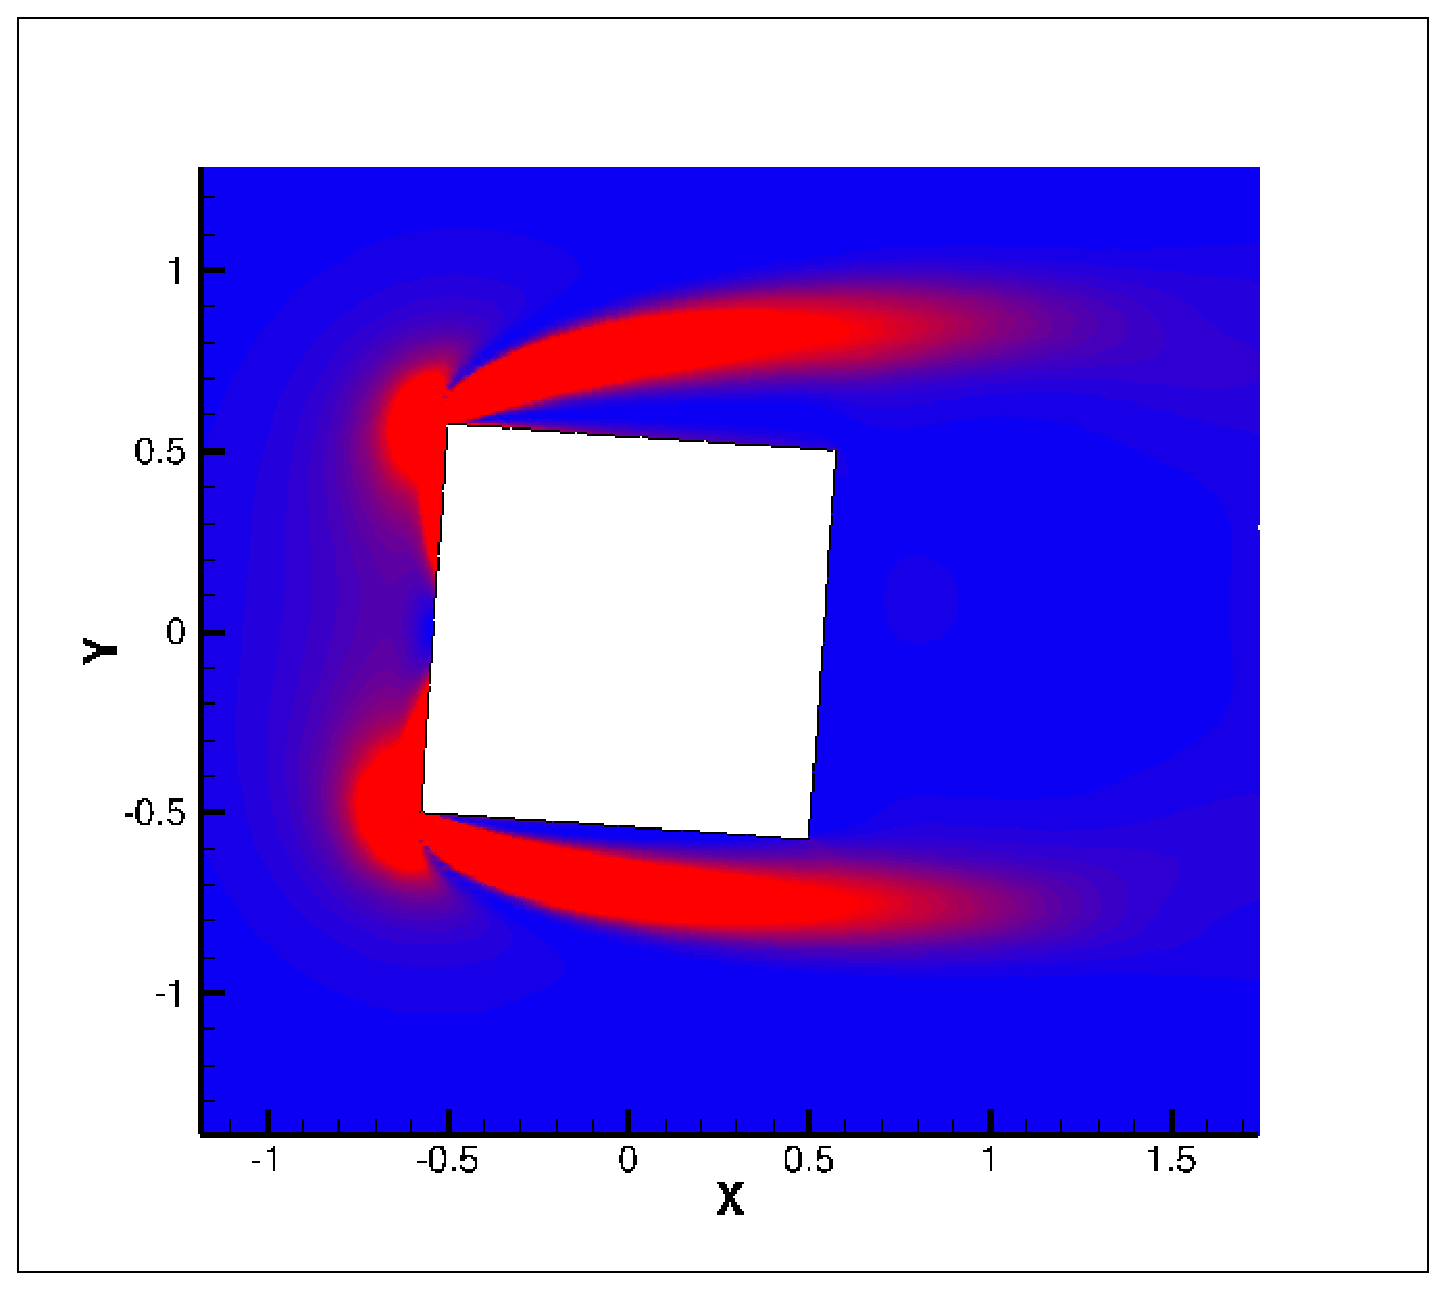
\includegraphics[width=0.33\unitlength]{./chapter-literature-revirw/fnp/square-4.eps}}
    \put(0.68,0.76){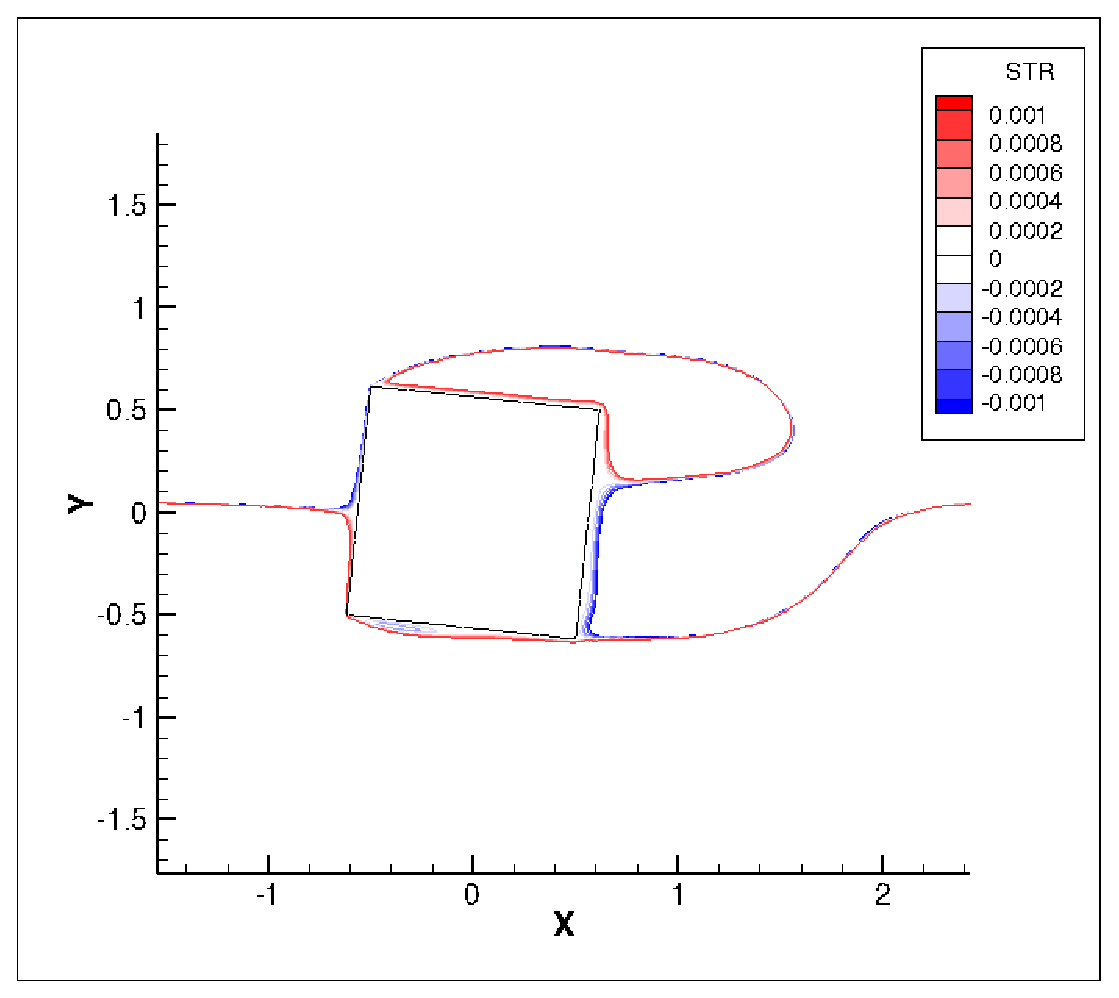
\includegraphics[width=0.33\unitlength]{.//chapter-literature-revirw/fnp/square-6.eps}}

   
    
    \put(0.0,0.735){(a)}    
    \put(0.34,0.735){(b)}
    \put(0.685,0.735){(c)}
  
  \end{picture}

  \caption{Stream functions of time averaged flow field on a stationary square section at $\reynoldsnumber=200$ at different incidence angles. (a) $2^{\circ}$ ($C_{y}$ increases),(b) $4^{\circ}$ ($C_{y}$ peaks) and (c) $2^{\circ}$ ($C_{y}$ decreases). The bottom shear layer comes closer to the bottom wall and reattaches as the angle of incidence increases.}
  \label{fig:shear_layers}
\end{figure}






Galloping is governed by the the shear layers created at the leading edge due to flow separation on the top and bottom corners of the bluff body. A common example is a square cross section as show in figure \ref{fig:shear_layers} which has been used widely in studies on galloping. Figure \ref{fig:shear_layers} shows the stream functions of time averaged (over a vortex shedding cycle) flow fields of stationary cross sections. The angle of incidence ($\theta$)increases clockwise from $2^{\circ}-6^{\circ}$. As $\theta$ is increased, the bottom shear layer comes closer to the wall of the body compared to the top shear layer (Figure \ref{fig:shear_layers} (a)). The shear layer nearer to the body crates higher suction compared to the shear layer at the opposite side. This pressure imbalance between the top and bottom sides of the body creates a downward force (i.e. the negative lift). As the angle is increased, the bottom shear layer becomes closer and therefore the pressure difference becomes grater leading to a higher $C_{y}$. The negative lift force becomes maximum when the shear layer near to the wall reattaches at the trailing edge (figure \ref{fig:shear_layers} (b)). As $\theta$ is further increased, the bubble in the bottom shear layer shrinks in size resulting the reduction of the pressure imbalance of the top and bottom surface leading to the reduction in $C_{y}$. This variation of \cy\ vs $\theta$ is presented in figure \ref{fig:lift_curves}. As the body is connected to an oscillatory system (discussed in section \ref{sec:exci-galloping}), this shear layer behaviour also harmonize with the cyclic behaviour of the system providing the driving force to the system so that the motion of galloping is sustained.



\subsection{Frequency response}
 
 It is clear that the cyclic motion of the shear layer harmonize with the mechanical system. Therefore, the frequency response should be then, the natural frequency of the system $\omega_{n}$ \citep{Paidoussis2010}. This is significantly different from the VIV mechanism, where the primary frequency comes from the periodic forcing of the vortex shedding. Hence, in the QSS model the natural frequency of the system could be identified as the frequency of oscillations. However, it should be  noted that this is valid on the regimes where the conditions discussed in section \ref{sec:QSS theory} are satisfied. 
 
 The experimental studies carried by \citet{bouclin:77} concluded at high reduced velocities with large inertia, the motion of the cylinder controls the frequency of the system rather than the vortex shedding. The structural damping has no effect provided that it is small. He also concluded that as the inertia and the reduced velocity gets lower, there is some interaction between vortex shedding and galloping. And at this region the frequency is mainly governed by the vortex shedding. 
 
 
 \subsection{Fluid mechanics governing the galloping response}
 
 As discussed in subsection \ref{subsec:c_y and shear layers} the driving force of a galloping system is the asymmetrical placement of the shear layers at either sides of the body. In consequence, it is clear that a significant afterbody is needed for the shear layer interaction to sustain galloping. \citet{Parkinson1974,Parkinson1989} and \citet{Bearman1987} have discussed well the importance of the length and the shape for galling in their reviews. It is also highlighted in \citet{Parkinson1974} that the most important physical parameters for galloping are the size relative to the characteristic hight and the shape of the afterbody. Manipulating the shape of the afterbody and thereby, manipulating the shear layer interactions with the body, gives the ability to control the galloping response. Thus, due to this reason work has been carried out on the response of galloping of different cross sectional shapes. 
 
 \citet{Blevins1990} provided a good comparison of the shapes which are prone to galloping based on the work by \citet{Parkinson1961}, \citet{Nakamura1975a} and \citet{Nakamura1977}. The reproduction of Blevins's data could be found in \citet{Paidoussis2010} presented in figure \ref{fig:par_diff_cross_sec}. 
    
 \begin{figure}
	
  \setlength{\unitlength}{\textwidth}

\fbox{
        \begin{picture}(1,1.2)(0,0.5)

      % % % Parkinson Data 

      \put(0.05,0.52){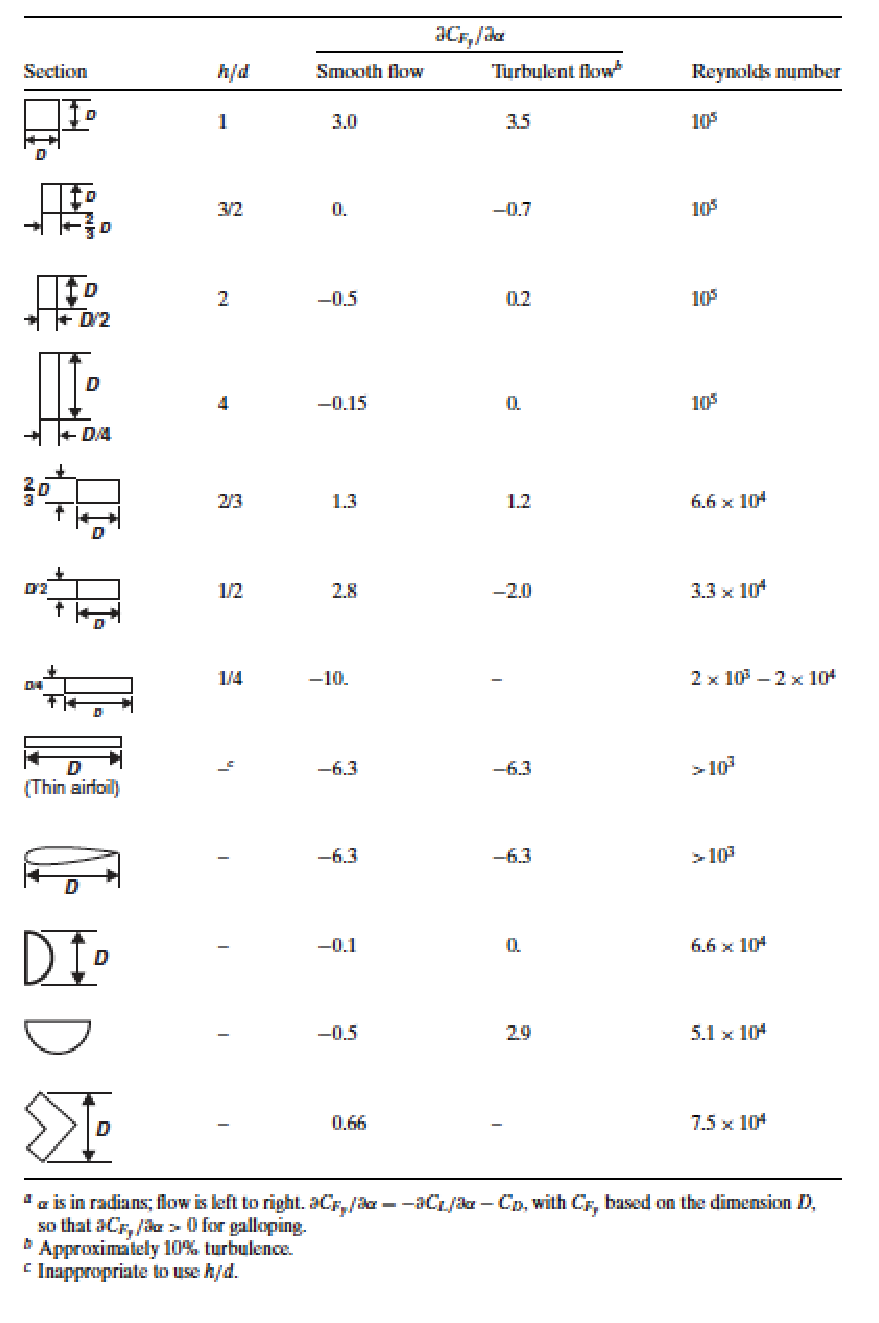
\includegraphics[width=0.75\unitlength]{./chapter-literature-revirw/fnp/per_cross_sec.eps}}
        


    \end{picture}
}
  \caption{ ``The transverse force coefficient for various sections in steady smooth or turbulent flow (after \citet{Blevins1990})" obtained from \citet{Paidoussis2010}. Here the induced angle is represented by $\alpha$ and the transverse force force coefficient is represented by $C_{fy}$. In order for galloping to sustain, the direction of both of these quantities should be same and thus have to satisfy the condition of $\frac{\partial C_{fy}}{\partial \alpha } >0$.}
    \label{fig:par_diff_cross_sec}
\end{figure}

 %vspace{10cm}

  
  
\citet{Naudascher1993}, \citet{Ruscheweyh1996}, \citet{Deniz1997} and \citet{Weaver2005} are some of the work done on different cross sectional shapes. \citet{Alonso2009} carried out wind tunnel tests on biconvex and rhomboidal cross sections. This study concluded that the galloping stability is dependent on the angle of attack. The aspect ratios where these cross sections were isolated. Studies were further carried out by Alonso for elliptical cross sections \citep{Alonso2010} which concluded that galloping is Reynolds number dependent for elliptical cross sections. The study triangular cross sections carried out by \citep{Alonso2005} isolated the angle of attacks where galloping is stained. The regions of stability for galloping at different angles of attack and the static force coefficients are presented in these studies with regards to the cross section involved. \citep{Luo1994} carried out an interesting study where the influence of the afterbody on galloping was investigated. The sides of a square section was chamfered gradually and two trapezoidal cross sections and one isosceles triangle was obtained. The \cy\ vs. $\theta$ plots revealed that the maximum value of \cy\ increased as the chamfering angle increased (i.e when the cross section was transformed from a square to a isosceles triangle). Anther interesting observation is that the angle which this maximum \cy\ increased as the chamfering angle increased.       


\subsection{Galloping as a mechanism of energy harvesting}

The focus on fluid-elastic galloping in the past was on understanding and developing methods to suppress it, due to the adverse effects on civil structures. However, recently, the focus of research has been redirected to develop mechanisms to excite galloping rather than suppressing it. This is due to the recent demand for alternate energy sources with minimal environmental impact. Thus, this demand for alternate energy have lead researchers to develop ways of extracting useful energy from flow induced vibrations.

Bernitsas and his group in the University of Michigan have made significant progress on using VIV as potential candidate for energy extraction. \cite{Bernitsas2008a-concept} introduced the concept of using VIV as a mode of energy extraction.The group have developed a device called VIVACE converter based on this concept. The work has been further expanded to focus on various aspects (such as Reynolds number effects, damping effects etc.) in \citet{Bernitsas2009,Raghavan2009,Raghavan2010a,Lee2011a}. This group have studied extensively on the effect of the mechanical parameters, the Reynolds number effects and the bottom boundary conditions of the VIVACE converter, in order to obtain efficient energy output using VIV as an energy harvesting mechanism. 

In contrast, the research carried out investigating the possibility of energy harvesting using fluid-elastic galloping is quite limited. \citet{Barrero-Gil2010a} conducted the pioneering study on energy harvesting using fluid-elastic galloping. The key consideration to investigate on galloping in this study was that unlike VIV fluid-elastic galloping was not dependent on a synchronisation or a ``lock-in" mechanism. Therefore, it could operate on a wide spectrum of frequencies giving fluid-elastic galloping an advantage over VIV as a mechanism of energy harvesting. \citet{vicente-Ludlam2014} showed that there is a link between the optimal electrical load resistance and the flow speed. However, it was identified that the understanding is a primary and therefore step-by-step research has to be conducted in order to properly understand the link between energy transfer in the galloping mechanism.

\subsection{Review summery and Objectives}

 It is clear that more investigations should be carried out on energy transfer of a galloping system, particularly to develop efficient energy harvesting system. More fundamental research is needed to explore the underpinning effects of mechanical and fluid dynamic parameters influencing the energy transfer of a galloping system to fill the gaps of the existing knowledge base. Thus, objectives of the current research were formulated in order to address these research gaps.
 
 Thus, this study was divided into two phases and objectives were defined 
 
 \subsection*{Phase 1: Understand the governing mechanical parameters of the system and isolate regions where a good power transfer could be obtained}
 
 \citet{Paidoussis2010} describes galloping as a ``velocity dependent damping controlled phenomenon". Yet, so far the scaling parameters used in studies are the traditional VIV parameters which are the damping ratio $\zeta$ and the reduced velocity \ustar\ \citep{Barrero-Gil2010a} which has a embedded frequency component. Thus following objectives were defined for this phase 
 
 \begin{itemize}
\item Formulate new set of scaling parameters the natural time-scales of the system.
\item Investigate the influence of these parameters on mean power transfer.
\item Isolate the regions where high power transfer could be obtained.
\item Investigate relationship between these new scaling parameters and the frequency response of the system. 
 \end{itemize}
 
    
  \subsection*{Phase 2: Understand the fluid mechanics of the system and optimise and control these mechanics to obtain a higher power transfer}
  
  \citet{Luo1994} showed that delaying shear layer reattachment could lead to higher peak $F_{y}$ at higher induced angles and therefore higher transverse velocities. Thus, from equation \ref{eqn:power}, it could be hypothesised that a higher mean power could be obtained by delaying the shear layer reattachment. Hence, the following objectives were defined for phase 2. 
  
  \begin{itemize}
  	\item Obtain QSS power data by systematically delaying the shear layer and investigate the influence on power.
  	\item Identify the relationship of involved fluid mechanics and the mean power output through analysis of the flow-filed.
  	\item Provide design considerations for a galloping energy extraction system through control of the shear layers. 
  \end{itemize}
 
 
 
 
 
 
 























  


    

     










